
\documentclass[11pt]{article}
\usepackage{standalone}
\usepackage[margin=0.75in, headheight=20pt]{geometry}

\usepackage{amsmath}
\usepackage{amsfonts}
\usepackage{amssymb}
\usepackage{mathtools}

\usepackage{tikz}
\usetikzlibrary{shadings,intersections}

\usepackage{caption,tabularx,booktabs}

\usepackage{rotating}

\usepackage[utf8]{inputenc}
\usepackage[english]{babel}
\setlength{\parindent}{2em}
\setlength{\parskip}{.25em}
\renewcommand{\baselinestretch}{1.0}

\usepackage{fancyhdr}
\pagestyle{fancy}
\rhead{ Clarke | Blostein | Queen's University}
\renewcommand{\headrulewidth}{0.4pt}
\renewcommand{\footrulewidth}{0.4pt}

\usepackage{courier}

\usepackage[]{algorithm2e}
\usepackage{mathrsfs}

\usepackage{etoolbox}
\patchcmd{\thebibliography}{\chapter*}{\section*}{}{}




\title{Performance Analysis of Semi-Orthogonal User Groups}
\author{J.E. Clarke, Dr. S.D. Blostein | Queen's University}
\date{Summer, 2018}

\begin{document}
	\maketitle
	\newpage
	\section{Introduction}
	    The objective of this paper is to devise a practical method for associating stations (STAs) to access points (APs) for application in IEEE 802.11 MU-MIMO downlink. Currently the 802.11 standard associates STAs with APs on a strongest signal first (SSF) basis \cite{IEEE80211}. While this method of association works well in sparsely populated networks, it is not necessarily the best choice in densely populated networks. Since the population of STAs and APs is unlikely to be uniformly spatially distributed throughout the local area network (LAN), the SSF association scheme is prone to overloading some APs while other APs that are within service range of STAs causing the bottleneck go under utilized.

Contrasting the naive SSF approach, it is theoretically conceivable that a globally optimal association solution in the sense of fairness-weighted sum rate might be found by way of a brute force search. In practice, however, the size of this search space grows very quickly. STAs must first be slotted into concurrent transmission groups (CTGs). Once the set of potential CTGs have been formed, each a set of potential associations is generated by considering each potential CTG associated with each AP. Effectively, this amounts to a cascading the result of one binomial coefficient into the argument of another. Thus, a brute force approach is completely intractable in practice.

The approach taken here is to place constraints on the formation of CTGs. More specifically, the candidate STAs for addition to CTGs are subjected to constraints on channel gain for any given channel in the group and minimum degree orthogonality between channel vectors associated with STAs in the CTG. CTGs formed subject to these constraints are referred to as semi-orthogonal user selection (SUS) groups. Semi-orthogonality has been the subject of various investigations including \cite{Swannack2005}, \cite{Yoo2006}. It has been shown in this work that by subjecting users (STAs in our case) to such norm and orthogonality constraints when forming SUS groups, MU-MIMO sum rate performance using beamforming is asymptotically optimal as the number of users becomes sufficiently large. Thus, we adopt a SUS approach as a method of limiting the search space of the optimal association problem while attempting to minimize the reduction in optimality of this more practical solution.

A spherical packing approach is adopted similar to that proposed by \cite{Swannack2005}. Motivation for using this approach is based on the flexibility of trading off the strictness of the channel norm and orthogonality requirements and probability of finding a SUS group that satisfies these constraints. Such flexibility is of particular interest in our context as it allows us to control the size of the association optimiziation search space as a function of expected SUS group sum rate.

The spherical packing approached developed by \cite{Swannack2005} is found to have limitations in terms of the tightness of SUS existence probability bounds. The looseness of this bound is clearly illustrated in this work by comparing these theoretical lower bounds on probability to numerically simulated values. This result is not unexpected, as the union bounds underpinning this lower bound become increasingly loose in some scenarios including large SUS group sizes and small number of transmit antennas.

The work shows that the looseness of these bounds can be mitigated by making use of widely linear processing operating on purely real transmitted data (ie. single dimensional constellations such as BPSK or M-PAM). It has been shown that such widely linear processing techniques used in conjunction with purely real constellations has (TODO: COMMENT ON MAJID'S RESULTS) 
    \section{System model}
        
\begin{figure}
    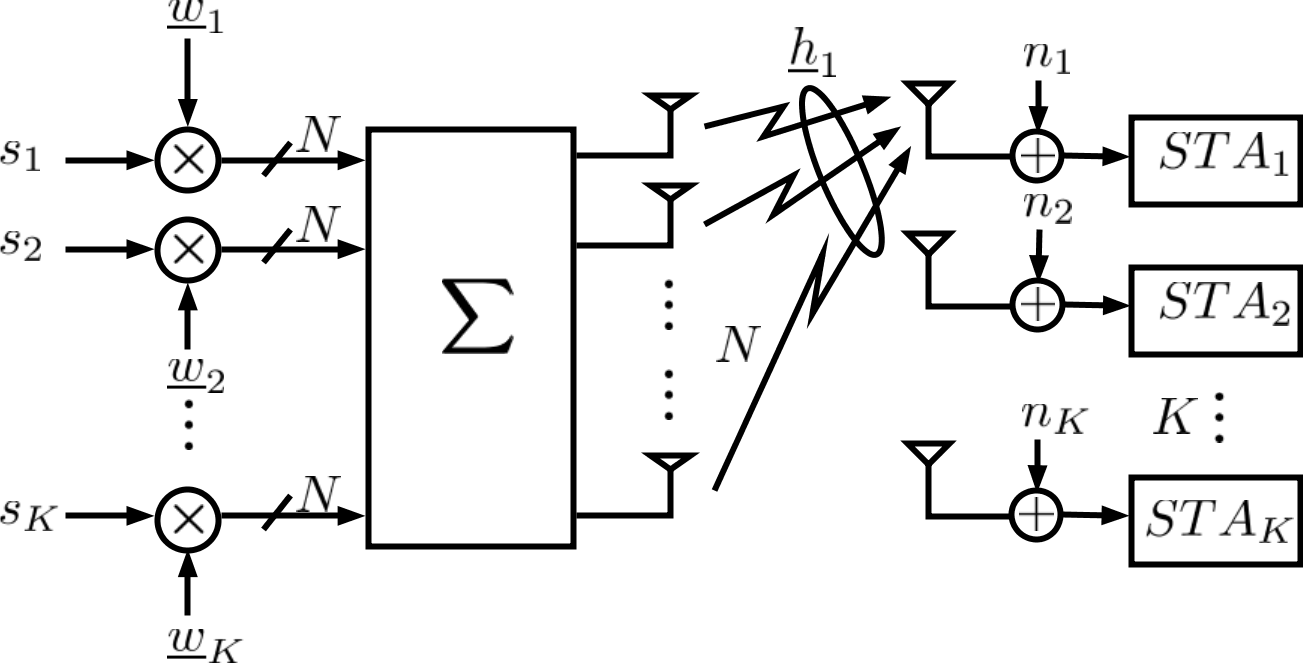
\includegraphics[width=12cm]{figs/system_desc.png}\\
    \caption{Block diagram of the system model.}
    \label{fig:sys_bd}
\end{figure}

    \section{Probability of SUS group existence}
        \subsection{Projecting vectors to points on spherical surface}\label{sec:chan_norm}
            In the MU-MIMO wireless context of interest, we have a MIMO transmitter with $N$ transmit antennas transmitting to $K$ single-antenna users. This topology means that the $i^{th}$ user has a  $N \times 1$ complex channel vector,$\underline{h}_i$, associated with it. That is, $\underline h_i\ \in \mathbb{C}^{1 \times N}$. A Rayleigh fading channel is assumed. Therefore each term in the channel vector $h_i$ follows a complex circularly symmetric iid normal distribution $\mathcal{N}_c(0,\frac{1}{N})$. It follows that the channel norm $\Vert \underline h_i \Vert^2$ follows a gamma distribution with the following parameters: $\Vert \underline h_i \Vert^2 \sim \mathcal{G}(2N,\frac{2}{N})$.

In order to formulate the problem as a sphere packing problem, channel vectors are assumed to be on the surface of a $N$-dimensional hyper-sphere in the complex domain, or a $2N$-dimensional hyper-sphere in the real domain. That is, the norms of each channel vector are assumed to be the same. This is evident from the definition of a hyper-sphere in $N$ dimensions:
\begin{equation}\label{eq:sphere_def}
    \begin{aligned}
        \mathcal{S}^{2N} = \lbrace \underline{h_i} \in \mathbb{R}^N \ : \ \Vert \underline{h_i} \Vert^2 = \rho \rbrace
    \end{aligned}
\end{equation}
where $\mathcal{S}^{2N}$ is the surface of a $2N$ hyper-sphere, $\underline{h}_i$ is a $N$-length complex vector that is being projected from the origin of the sphere, $\mathcal{O}$, to its surface, and $\sqrt{\rho}$ is the radius of the sphere. Without loss of generality, a sphere with radius of $\sqrt{\rho}$ can be mapped on a one-to-one basis to a sphere with radius $\rho$. Such a mapping is assumed for convenience.

In the case of a wireless channel experiencing deterministic path loss and Rayleigh fading, it is not practical to assume that all vectors have the same norm. If path loss is not exactly the same for each vector, the channel norms will differ between vectors (implying they would fall on the surface of spheres with different radii, or some other arbitrary shape). Similarly, the stochastic nature of the channel vectors, due to fading, will have the same effect.

However, if we assume channel state information at the transmitter (CSIT), the path loss can be estimated and accounted for (neglecting any estimation error in path loss, and assuming power control). Furthermore, the probability that $\Vert \underline{h_i} \Vert^2$ exists in the spherical shell defined by lower and upper radii, $\rho^-$ and $\rho^+$, respectively, is non-zero and can be easily calculated as a function of fading statistics and $\rho^-,\ \rho^+ $. An illustration of the members of this family of spheres is illustrated in Fig. $\ref{fig:concentric_sphere}$.

\begin{figure}
    \centering
    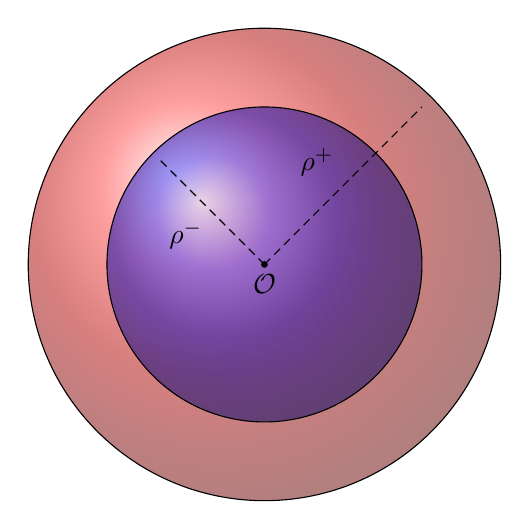
\begin{tikzpicture}
      \coordinate (O) at (0,0);
      
      % outer ball background color
      \shade[ball color = red, opacity = 0.5] (0,0) circle [radius = 3cm];
    
      %outer ball ball
      \draw (O) circle [radius=3cm];
    
      % inner ball background color
      \shade[ball color = blue, opacity = 0.5] (0,0) circle [radius = 2cm];
    
      % inner ball
      \draw (O) circle [radius=2cm];
      % label of ball center point
      \filldraw (O) circle (1pt) node[below] {$\mathcal{O}$};
    
      % radius for inner ball
      \draw[densely dashed] (O) to [edge label = $\rho^-$] (-1.33,1.33);
      % radius for outer ball
      \draw[densely dashed] (O) to [edge label = $\rho^+$] (2,2);
      
    
    \end{tikzpicture}
      \caption{Concentric hyper-spheres of radii $\rho^-,\rho^+$. Channel norms are restricted to this range in order to project vectors onto the surface of a hyper-sphere of constant radius. In order to pessimistically lower bound orthogonality probabilities, the larger radius of $\rho^+$ is chosen. The probability channel norms will fall into this range can be described in terms of channel fading statistics.}
    \label{fig:concentric_sphere}
\end{figure}
  
The CDF of the channel norm will be denoted by $F_{\Vert\underline{hi}\Vert^2}(m,\rho)$, where $\rho$ are realizations of the random variable formed by the channel norm. Each term in the $N$-length vector, $\underline{h}_i$ is represented by two iid normal random variables: one for the real part and one for the imaginary part. When forming the L2 norm of the $N$-length vector, each multiplication forms a sum of length four where each of the arguments of the sum are a product of two random variables. Namely, the sum takes the form real$\cdot$real + real$\cdot$imaginary + imaginary$\cdot$real + imaginary$\cdot$imaginary. Therefore we have a four-term sum of squared normal random variables. Therefore, this sum of squares results in a Gamma distribution with four degrees of freedom, the CDF of the resulting random variable becomes
\begin{equation}\label{eq:ch_sq_cdf_chan}
    \begin{aligned}
        F_{\Vert\underline{hi}\Vert^2}(\rho;m)& = \Gamma_n(2m,m\rho)\\
        &= Pr[\Vert\underline{h}_i\Vert^2 \leq \rho] \ \ ,
    \end{aligned}
\end{equation}
where $\Gamma_n(\cdot)$ is the incomplete normalized gamma function.

The probability that $\Vert\underline{h}_i\Vert^2$ lands in the shell between radii $\rho^+,\ \rho^-$,  is given by the subtraction of the respective CDF expressions:
\begin{equation}\label{eq:p_s}
    \begin{aligned}
        p_s = \Gamma_n(2N,N\rho^-) - \Gamma_n(2N,N\rho^+)
    \end{aligned}
\end{equation}

The issue of resolving the projection of channel vectors onto the surface of a sphere is still not entirely resolved: we have only described the probability the vectors will exist in a shell defined by upper and lower bounding radii. In order to pessimistically bound orthogonality analysis in the upcoming discussion, it is assumed that all the channel norms that exist in the shell are equal to $\rho^+$. This approach implies a trade-off between probability of channel norms existence and accuracy of orthogonality analysis: as ${(\rho^+-\rho^-)\rightarrow 0},\ p_s\rightarrow 0$; however, as  $(\rho^+-\rho^-)$ grows, so does the inaccuracy in orthogonality analysis.



        \subsection{$\epsilon$-orthogonality of points on spherical surface}\label{sec:spherical_caps}
            Orthogonality between pairs of vectors can be interpreted geometrically on the surface of a $2N$-dimensional hyper-sphere, given by $\mathcal{S}^{2N}$,  in terms of spherical caps. A spherical cap is formed on the surface of the hyper-sphere of radius $\rho^+$ by by first extending the channel vector $\underline{h_i}$ onto the spherical surface as described in Section \ref{sec:chan_norm}. When $\underline{h_i}$ is extended to the spherical surface, it defines a point $\mathcal{P}_i$ that lives on the surface of the sphere. Then a cone, with its apex at $\mathcal{O}$, with half angle $\theta$, centered along the axis of $\underline{h_i}$ is intersected with the spherical surface. This intersection defines a spherical cap, $\mathcal{C}_i$. This process is illustrated in Fig. \ref{fig:spherical_cap}. 

Spherical caps can be used to describe the the degree of orthogonality between a given vector $\underline{h_i}$ and an arbitrary vector $\underline{h_j}$ by viewing $\mathcal{C}_i$ as a `keep-out zone' $\forall \  \mathcal{P}_j,\ j\neq i \ \in \mathcal{S}^{2N}$. More formally:
\begin{equation}\label{eq:cap_orth}
    \begin{aligned}
    \mathcal{P}_j \not\in \mathcal{C}_i\ \forall j\neq i \in \mathcal{S}^{2N}
    \end{aligned}
\end{equation}
It is important to realize that $\mathcal{C}_i$ is a function of $\theta \in [0,\frac{\pi}{2}]$. That is, $\theta$ is a parameter that describes the degree of orthogonality between vectors: as $\theta \rightarrow \frac{\pi}{2}$ vectors that comply with Eq. (\ref{eq:cap_orth}) are increasingly orthogonal to $\underline{h_i}$. When the condition given in Eq. (\ref{eq:cap_orth}) is satisfied, $\underline{h_i}$ and $\underline{h_j}$ are said to  be $\epsilon$-orthogonal. That is, these two vectors are $\epsilon$-orthogonal to each other to a minimum degree given by the parameter, $\epsilon$.

We can relate the spherical cap interpretation of orthogonality to inner products between vectors on a pair-wise basis. A geometric interpretation is shown in Fig. \ref{fig:cap_triangle}. In this figure, we introduce $\epsilon$, which is related to $\rho^+$, $\theta$:
\begin{equation}\label{eq:epsilon}
    \begin{aligned}
    \epsilon = \rho^+\cos{\theta} \ \ .
    \end{aligned}
\end{equation}
We form the unit vector along $\underline{h_i}$:
\begin{equation}\label{eq:unit_vec}
    \begin{aligned}
    \Hat{\underline{h_i}} = \frac{\underline{h_i}}{\sqrt{\rho^+}} \ \ .
    \end{aligned}
\end{equation}
Thus we can form the inner product between $\Hat{\underline{h_i}}$ and $\Hat{\underline{h_j}}$:
\begin{equation}\label{eq:inner_prod}
    \begin{aligned}
    <\Hat{\underline{h_i}},\Hat{\underline{h_j}}> &= \vert \Hat{\underline{h_j}}^H\Hat{\underline{h_i}} \vert\\
    &\leq \frac{\epsilon}{\rho^+} \ \ .
    \end{aligned}
\end{equation}
The scenario shown in Fig. \ref{fig:cap_triangle} is the case where $\underline{h_j}$ is as close to living entirely in $\mathcal{C}_i$ without doing so. Namely, it shows the case of the equality shown in Eq. (\ref{eq:inner_prod}) where $\mathcal{P}_j$ lives on the circular boundary of $\mathcal{C}_i$ (ie. $\mathcal{P}_j$ may live partially in $\mathcal{C}_i$, but not entirely.). Furthermore, the inequality in Eq. (\ref{eq:inner_prod}) does not hold if $\mathcal{P}_j\in \mathcal{C}_i$.
\begin{figure}
\centering
    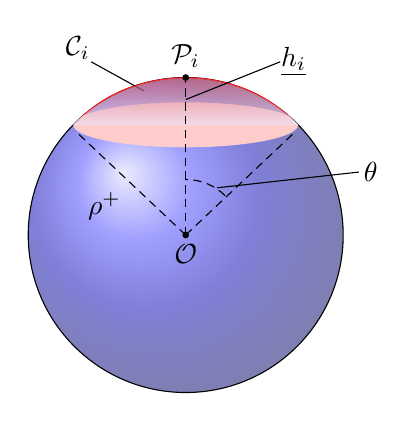
\begin{tikzpicture}%[font = \sansmath]
        %define origin, 1-height of cone, radius
        \coordinate (O) at (0,0);
        \def\r{2}
        \def\H{.6}
        
        \begin{scope}
        % ball background color
        \shade[ball color = blue, opacity = 0.5] (0,0) circle [radius = \r];
        
        % cone
        \begin{scope}
            \def\rx{0.71}% horizontal radius of the ellipse
            \def\ry{0.15}% vertical radius of the ellipse
            \def\z{0.725}% distance from center of ellipse to origin
        
            \path [name path = ellipse]    (0,\z) ellipse ({\rx} and {\ry});
            \path [name path = horizontal] (-\rx,\z-\ry*\ry/\z)
                                        -- (\rx,\z-\ry*\ry/\z);
            \path [name intersections = {of = ellipse and horizontal}];
        
            %% radius to base of cone in ball
            %\draw[fill = gray!50, gray!50] (intersectioN) -- (0,0)
            %  -- (intersection-2) -- cycle;
            %% base of cone in ball
            %\draw[fill = gray!30, densely dashed] (0,\z) ellipse ({\rx} and %{\ry});
        \end{scope}
        
        % label of cone
        %\draw (0.25,0.4) -- (0.9,0.1) node at (1.05,0.0) {$q$};
        
        % ball
        \draw (O) circle [radius=2cm];
        
        % label of ball center point
        \filldraw (O) circle (1pt) node[below] {$\mathcal{O}$};
        
        % radius
        \draw[densely dashed] (O) to [edge label = $\rho^+$] (-1.4,1.32);
        \draw[densely dashed] (O) -- (1.4,1.32);
        %label colatitude angle
        \draw[densely dashed] (0.5,0.5) arc [start angle = 45, end angle = 90, x radius = 7mm, y radius = 7mm];
        \draw (2.2, 0.8) -- (0.4, 0.6) node at (2.35,0.8) {$\theta$};
        
        % cut of ball surface
        \draw[red] (-1.35,1.47) arc [start angle = 140, end angle = 40, x radius = 17.6mm, y radius = 14.75mm];
        %\draw[red, densely dashed] (-1.36,1.46) arc [start angle = 170, end angle = 10,
        x radius = 13.8mm, y radius = 3.6mm];
        %\draw[red] (-1.29,1.52) arc [start angle=-200, end angle = 20,
        x radius = 13.75mm, y radius = 3.15mm];
        
        % label of cut of ball surface
        \draw (-1.2,2.2) -- (-0.53,1.83) node at (-1.37,2.37) {$\mathcal{C}_i$};
        
        %shade the spherical cap
        \begin{scope}
            %clip the shading outside the ball
            \clip ({\r*cos(-90)},{\r*sin(-90)}) arc [start angle=-90,end angle=270,radius=\r];
            %draw the disk    
            \fill[red!20] (0,{\r-\H}) circle [x radius={sqrt(\r^2-(\r-\H)^2)}, y radius={0.2*sqrt(\r^2-(\r-\H)^2)}];
            %shade the disk
            \shade[top color=red!70!gray,bottom color=red!10!blue!10!,opacity=0.6]  ({\r},{1.1*\r}) rectangle ++({-2*\r},{-0.1*\r-\H});
        \end{scope}
    
        %draw channel vector
        \draw[densely dashed] (O) -- (0,2);
        %label channel vector
        \draw (1.2,2.2) -- (0,1.72) node at (1.37,2.2) {$\underline{h_i}$};
        % label of ball center point
        \filldraw (0,2) circle (1pt) node[above] {$\mathcal{P}_i$};
        \end{scope}
    \end{tikzpicture}
    
    \caption{Surface of hyper-sphere in 2$N$ dimensions. A spherical cap, $\mathcal{C}_i$ is shown (shaded in red). $\mathcal{C}_i$ is formed by projecting the channel vector, $\underline{h_i}$, onto the spherical surface. A colatitude angle of $\theta$ and radius of $\rho^+$ are assumed in forming $\mathcal{C}_i$. Alternatively, $\mathcal{C}_i$ can also be interpreted as the cap formed by intersecting a cone of half-angle $\theta$ with the spherical surface.}
    \label{fig:spherical_cap}
\end{figure}

\begin{figure}
\centering
    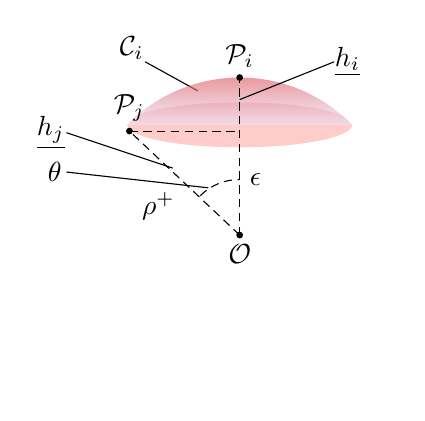
\begin{tikzpicture}%[font = \sansmath]
        %define origin, 1-height of cone, radius
        \coordinate (O) at (0,0);
        \def\r{2}
        \def\H{.6}
        
        \begin{scope}
        % ball background color

        \begin{scope}
            \def\rx{0.71}% horizontal radius of the ellipse
            \def\ry{0.15}% vertical radius of the ellipse
            \def\z{0.725}% distance from center of ellipse to origin
        
            \path [name path = ellipse]    (0,\z) ellipse ({\rx} and {\ry});
            \path [name path = horizontal] (-\rx,\z-\ry*\ry/\z)
                                        -- (\rx,\z-\ry*\ry/\z);
            \path [name intersections = {of = ellipse and horizontal}];
        
            % radius to base of cone in ball
            %\draw[fill = gray!50, gray!50] (intersectioN) -- (0,0) -- (intersection-2) -- cycle;
            % base of cone in ball
            %\draw[fill = gray!30, densely dashed] (0,\z) ellipse ({\rx} and %{\ry});
        \end{scope}
        
        % label of cone
        %\draw (0.25,0.4) -- (0.9,0.1) node at (1.05,0.0) {$q$};

        % label of ball center point
        \filldraw (O) circle (1pt) node[below] {$\mathcal{O}$};
        
        % radius
        \draw[densely dashed] (O) to [edge label = $\rho^+$] (-1.4,1.32);
        %\draw[densely dashed] (O) -- (1.4,1.32);
        %label colatitude angle
        \draw[densely dashed] (-0.5,0.5) arc [start angle = 135, end angle = 90, x radius = 7mm, y radius = 7mm];
        \draw (-2.2, 0.8) -- (-0.4, 0.6) node at (-2.35,0.8) {$\theta$};
        
       
        %\draw[red, densely dashed] (-1.36,1.46) arc [start angle = 170, end angle = 10,
        x radius = 13.8mm, y radius = 3.6mm];
        %\draw[red] (-1.29,1.52) arc [start angle=-200, end angle = 20,
        x radius = 13.75mm, y radius = 3.15mm];
        
        % label of cut of ball surface
        \draw (-1.2,2.2) -- (-0.53,1.83) node at (-1.37,2.37) {$\mathcal{C}_i$};
        
        %shade the spherical cap
        \begin{scope}
            %clip the shading outside the ball
            \clip ({\r*cos(-90)},{\r*sin(-90)}) arc [start angle=-90,end angle=270,radius=\r];
            %draw the disk    
            \fill[red!20] (0,{\r-\H}) circle [x radius={sqrt(\r^2-(\r-\H)^2)}, y radius={0.2*sqrt(\r^2-(\r-\H)^2)}];
            %shade the disk
            \shade[top color=red!70!gray,bottom color=red!10!blue!10!,opacity=0.6]  ({\r},{1.1*\r}) rectangle ++({-2*\r},{-0.1*\r-\H});
        \end{scope}
    
        %draw channel vector
        \draw[densely dashed] (O) -- (0,2);
        
        %epsilon label
        \draw node at (0.2,0.7) {$\epsilon$};
        
        %label channel vector
        \draw (1.2,2.2) -- (0,1.72) node at (1.37,2.2) {$\underline{h_i}$};
         %label channel vector
        \draw (-2.2, 1.3) -- (-0.85,0.85) node at (-2.4,1.3) {$\underline{h_j}$};
        
        % label of ball center point
        \filldraw (0,2) circle (1pt) node[above] {$\mathcal{P}_i$};
        
        % label of point from second vector
        \filldraw (-1.4,1.32) circle (1pt) node[above] {$\mathcal{P}_j$};
        %draw top part of right triangle
        \draw[densely dashed] (-1.4,1.32) -- (0,1.32);
        \end{scope}
    \end{tikzpicture}
    
    \caption{Relationship between spherical cap and inner product of vectors $\underline{h_i},\ \underline{h_j}$}. $\mathcal{P}_j$ lives outside of $\mathcal{C}_i$, however, it is as close as it can be to the cap without living inside it.
    \label{fig:cap_triangle}
\end{figure}
            Following from the discussion of projecting vectors onto the spherical surface, and defining spherical caps associated with these points, we now extend these concepts the scenario of packing caps onto the surface of the sphere. In this scenario, we assume that vectors are randomly projected onto the surface of the sphere with a uniform density independently from each-other. We would like to know the probability that we can pack $l$ spherical caps of colatitude angle $\theta$ onto the surface of the sphere conditioned on the projection of such vectors onto the surface (as described in Section \ref{sec:chan_norm}). Channel vectors are chosen from a set $\mathsf{A},\ \vert \mathsf{A}\vert = l$ More formally:
\begin{equation}\label{eq:p_perp_cdl}
    \begin{aligned}
        p_\perp &= Pr[\underset{i \in\mathsf{A}}{\cap} \mathcal{P}_j\not\in\mathcal{C}_i\ \forall j\neq i\in\mathsf{A}\ \vert\ \rho^-\leq  \Vert \underline{h_i} \Vert^2 \leq \rho^+,\ \theta ]\\
        &\geq Pr[\underset{i \in\mathsf{A}}{\cap} \mathcal{P}_j\not\in\mathcal{C}_i\ \forall j\neq i\in\mathsf{A}\ \vert\ \Vert \underline{h_i} \Vert^2 = \rho^+,\ \theta ]
    \end{aligned}
\end{equation}
The expression given in Eq. (\ref{eq:p_perp_cdl}) may alternatively be described as the probability that no vector in $\mathsf{A}$ lives in any other vector's spherical cap on the surface $\mathcal{S}^{2N}$, given the vectors live on this surface and a colatitude angle $\theta$ for the cap. The inequality in Eq. ($\ref{eq:p_perp_cdl}$) can be explained by the assumed channel norm length of $\rho^+$ for each vector. The channel norms are assumed to be larger than they actually are. Therefore, when the inner product is formed, the vectors are assumed to be longer than they actually are. Therefore, their projections onto each-other will be larger than they should be. Thus, the orthogonality constraint is harder to meet.

The probability $p_\perp$ can be expressed in terms of the fractional area of $\mathcal{S}^{2N}$. The probability that any two pair-wise vectors are orthogonal is given by fraction of the area remaining on $\mathcal{S}^{2N}$ after adding $l-1$ cap to the surface. Let $\Omega_{2N}(\rho^+,\theta)$ denote the area of a spherical cap of colatitude angle $\theta$. Therefore the probability that any two vectors are orthogonal on a pair-wise basis is:
\begin{equation}\label{eq:delta_c}
    \begin{aligned}
        \delta_c(\theta,2N) = 2\frac{\Omega_{2N}(\rho^+,\theta)}{\Omega_{2N}(\rho^+,\pi)} \ \ .
    \end{aligned}
\end{equation}
Thus, the fractional area remaining on $\mathcal{S}^{2N}$ after considering one pair of vectors (ie. $\vert \mathsf{A} \vert = 2$) can be interpreted as a probability given by 
\begin{equation}\label{eq:p_perp_l2}
    \begin{aligned}
        p_{\perp,l=2} = 1-\delta_c(\theta,2N) \ \ .
    \end{aligned}
\end{equation}

We would like to consider groups of larger sizes (ie. $l> 2$). However, we have the difficulty of determining whether or not the the spherical caps overlap each other. It is important to realize that if the spherical caps $\mathcal{C}_i$ and $\mathcal{C}_j$ intersect each other, it is still possible the vectors are $\epsilon$-orthogonal. However, we know that if $\mathcal{C}_i\cap\mathcal{C}_j = \lbrace \emptyset \rbrace$ the vectors are $\epsilon$-orthogonal since there is no way $\mathcal{P}_j\in\mathcal{C}_i$: the cap $\mathcal{C}_j$ of non-zero radius prevents this from happening. In this way we can define a lower bound on $p_\perp$, by recalling each vector is projected on the sphere independent from all other vectors, and by assuming each cap is the same size and does not intersect any other cap, the union bound becomes:
\begin{equation}\label{eq:p_perp}
    \begin{aligned}
        p_{\perp} \geq (1-\delta_c(\theta,2N))^{l-1} \ \ .
    \end{aligned}
\end{equation}
It is important to note that the union bound used in Eq. (\ref{eq:p_perp}) becomes overly pessimistic as the surface of the sphere fills up with caps. The bound does not allow for any caps to intersect at all. However, in reality, it is alright for caps to intersect each other so long as the intersection is not so large that $\mathcal{P}_j\in\mathcal{C}_i$. Allowing some intersection between caps makes packing the sphere much easier as the surface fills up. Therefore for small $N$, large $l$, and/or large $\theta$ the bound in Eq. (\ref{eq:p_perp}) is not expected to be tight.

It has been shown in \cite{Li2011} that the $\delta_c$ function can be realized in terms of an incomplete regularized beta function. Let $\text{I}_z(a,b)$ be the incomplete regularized Beta function. The Beta function is given by the integral:
\begin{equation}\label{eq:beta}
    \begin{aligned}
        \text{B}(a,b) = \int_0^1 t^{b-1}(1-t)^{a-1}dt; \ a>0,\ b>0  \ \ .
    \end{aligned}
\end{equation}

Similarly, the incomplete Beta function is given by
\begin{equation}\label{eq:beta_inc}
    \begin{aligned}
        \text{B}_z(a,b) = \int_0^z t^{b-1}(1-t)^{a-1}dt; \ a>0,\ b>0,\ z>0 \ \ ,
    \end{aligned}
\end{equation}
or alternatively through the integral, by making the use of a reparametrization to a polar coordinate system:
\begin{equation}\label{eq:beta_inc_sin}
    \begin{aligned}
        \text{B}_{\sin^2\theta}(\frac{N+1}{2},\frac{1}{2}) = 2\int_0^\theta \sin^N (\phi)\ d\phi; \ a>0,\ b>0,\ \theta>0 \ \ .
    \end{aligned}
\end{equation}

Finally the incomplete regularized function is given by
\begin{equation}\label{eq:beta_inc_reg}
    \begin{aligned}
        \text{I}_z(a,b) = \frac{\text{B}_z(a,b)}{\text{B}(a,b)} \ \ .
    \end{aligned}
\end{equation}

We will also make use of the expression for the surface area of an entire hyper-sphere in $N$ dimensions in terms of the Gamma function:
\begin{equation}\label{eq:omega_gamma}
    \begin{aligned}
        \Omega_N(\rho^+,\pi) = \frac{2\pi^{N/2}}{\Gamma(N/2)}(\rho^+)^{N-1} \ \ .
    \end{aligned}
\end{equation}

As is illustrated by Li in \cite{Li2011}, the area of a spherical cap in $N$ dimensions can be calculated by integrating the surface of a sphere in $N-1$ dimensions along the arc of a great circle with radius $\rho^+\sin\phi$, where the arc element along the great circle is given by $\rho^+d\phi$. This integral can be expressed in terms of the Beta function given above.
\begin{equation}\label{eq:cap_integral}
    \begin{aligned}
        \Omega_N(\rho^+,\theta) &= \int_0^\theta \Omega_{N-1}(\rho^+\sin\phi,\pi)\ \rho^+d\phi\\
        &= \frac{2\pi^{N-1/2}}{\Gamma(N-1/2)}(\rho^+)^{N-1}  \int_0^\theta \sin^{N-2}(\phi)d\phi\\
        &= \frac{1}{2} \Omega_N(\rho^+,\pi)\  \text{I}_{\sin^2(\theta)}\bigg(\frac{N-1}{2},\frac{1}{2}\bigg)
    \end{aligned}
\end{equation}
Therefore, comparing the expressions in Eqs. (\ref{eq:cap_integral}), (\ref{eq:delta_c}), we arrive at the following expression for $\delta_c$ in terms of the incomplete regularized Beta function:
\begin{equation}\label{eq:delta_c_beta}
    \begin{aligned}
        \delta_c(\theta,2N) = \text{I}_{\sin^2(\theta)}\bigg(\frac{2N-1}{2},\frac{1}{2}\bigg) \ \ .
    \end{aligned}
\end{equation}

Thus, the bound on $p_\perp$ from Eq. (\ref{eq:p_perp}) can be expressed in terms of $\text{I}_{\sin^2(\theta)}$:
\begin{equation}\label{eq:p_perp_beta}
    \begin{aligned}
        p_{\perp} \geq \bigg(1-\text{I}_{\sin^2(\theta)}\bigg(\frac{2N-1}{2},\frac{1}{2}\bigg)\bigg)^{l-1} \ \ .
    \end{aligned}
\end{equation}
        \subsection{$\epsilon$-orthogonal group existence probability}
            In Section \ref{sec:chan_norm} we described a method of approximately projecting channel vectors onto a spherical surface. In Section \ref{sec:spherical_caps} we used the event of this projection as a condition for developing a probability that a set of $l$ vectors, $\mathsf{A}$, is $\epsilon$-orthogonal. In this section we set out to extend these results further by considering a larger set of candidate vectors, $\mathsf{C} \ :\ \vert \mathsf{C} \vert = m >l$. This result is particularly useful because it allows us to consider the probability that we can find a group of $l$ vectors that are $\epsilon$-orthogonal as a function of the number of candidates we consider, $n$. One would expect that as more candidates are considered for addition to an $\epsilon$-orthogonal group of size $l$, the probability that such a group meets the constraints and attains minimum size $l$ increases with $n$. However, as more candidates are considered, the complexity associated with forming the $\epsilon$-orthogonal group also increases. In such a way we can trade off complexity for performance.

We can describe the collection of $\epsilon$-orthogonal sets (user groups) using the criteria developed in the previous sections. Let $\mathscr{S}_\epsilon$ be a collection of $\epsilon$-orthogonal sets. $\mathscr{S}_\epsilon$ is formed by testing all subsets of the set of candidate vectors, $\mathsf{A}\subset\mathsf{C}\ : \ \vert \mathsf{A} \vert = l$, against the channel norm and orthogonality constraints previously developed. Thus, $\mathscr{S}_\epsilon$ is a collection of $l$-length sets. The vectors contained within each of these $l$-length sets are mutually $\epsilon$-orthogonal. In the case that $\mathscr{S}_\epsilon = \lbrace \emptyset \rbrace$, no $\epsilon$-orthogonal sets of cardinality $l$ exist in the set of candidate vectors $\mathsf{C}$. This can be expressed more formally as:
 \begin{equation}\label{eq:S_e}
    \begin{aligned}
        \mathscr{S}_\epsilon = \lbrace \mathsf{A}\ \big|\ | \underline{h_j}^H\underline{h_i} |\ <\ \epsilon \ \text{;} \ \rho^-<\Vert \underline{h_i} \Vert^2 < \rho^+\ \forall \ i \neq j \in \mathsf{A} \rbrace \ \forall \mathsf{A}\subset \mathsf{C} \ \ .
    \end{aligned}
\end{equation}

The purpose of this discussion is to provide an expression for the probability that at least one such set exists, that is, $Pr[\mathscr{S}_\epsilon \neq \lbrace \emptyset \rbrace]$. We adopt the following notation to describe this probability.
 \begin{equation}\label{eq:p_epsilon}
    \begin{aligned}
        p_\epsilon = Pr[\mathscr{S}_\epsilon \neq \lbrace \emptyset \rbrace]
    \end{aligned}
\end{equation}
More specifically, we want to describe $p_\epsilon$ as a function of $l,\ n,\ \theta$. In order to work up to this result, let us first consider the case that $n=l$. In this case, there is only one non-null subset of $\mathsf{C}$, namely $\mathsf{C}$ itself. Therefore, the existence probability of $\epsilon$-orthogonal set can be stated in terms of Eqs. (\ref{eq:p_s}), (\ref{eq:p_perp_cdl} or \ref{eq:p_perp_beta}) by recalling that $p_s$ is independent of $p_\perp$:
 \begin{equation}\label{eq:p_epsilon_l}
    \begin{aligned}
        p_{\epsilon,l=n} = p_\perp p_s^l \ \ .
    \end{aligned}
\end{equation}

However, in the case that $n>l$, we must now consider more than one subset of $\mathsf{C}$. In order to do so, we first realize that since the vectors are independent, the probability that $K_{\rho^+}$ vectors will fall in the spherical shell defined by $\rho^-,\ \rho^+$ is given by a binomial distribution.
 \begin{equation}\label{eq:K_rho}
    \begin{aligned}
        Pr[K_{\rho^+} = l] = \binom{n}{l}p_s^l(1-p_s)^{(n-l)}
    \end{aligned}
\end{equation}

Next, we introduce the indicator random variable which returns a binary value indicating whether or not $\mathsf{A}\in \mathscr{S}_\epsilon$:
 \begin{equation}\label{eq:orth_indicator}
    \begin{aligned}
        \textbf{1}_{\mathsf{A}} = 
        \begin{cases}
            1,& \text{if } \mathsf{A} \in \mathscr{S}_\epsilon\\
            0,              & \text{otherwise}
        \end{cases} \ \ .
    \end{aligned}
\end{equation}

The number of $\epsilon$-orthogonal sets in the collection $\mathscr{S}_\epsilon$ may be expressed in terms of a sum of these indicator variables:
 \begin{equation}\label{eq:indicator_sum}
    \begin{aligned}
        K_\epsilon^{(l)} = \sum_{\mathsf{A}\subset\mathsf{C}}1_{\mathsf{A}} \ : \ \vert \mathsf{A} \vert = l \ \ .
    \end{aligned}
\end{equation}

We can now expand on the expression given in Eq. (\ref{eq:p_epsilon}) in terms of Eqs. (\ref{eq:indicator_sum}, \ref{eq:K_rho}). First we realize that we want the union of events corresponding to the existence of group sizes in the range $l\leq j \leq n$. We then form the probability of these events as the product of the probability associated with $j$ vectors existing in the shell (see Eq. (\ref{eq:K_rho})) and the probability that $K_\epsilon^{(l)} > 0$ conditioned on the existence of $j$ vectors in the shell. Note Eq.   ($\ref{eq:p_epsilon}$) is equivalent to $Pr[ K_\epsilon^{(l)} \neq 0]$.
 \begin{equation}\label{eq:p_epsilon_sum}
    \begin{aligned}
        p_{\epsilon,l,n} = \sum_{j=l}^n Pr[K_{\rho^+} = j] \cdot Pr[ K_\epsilon^{(l)} >0 \ \vert \ K_\rho^+ = j] \ \ ,
    \end{aligned}
\end{equation}
while we have useful expression for the first term in the sum, we still require a tractible expression for the second term in this sum. More specifically, we look to find an espression for the probability associated with the sum of random indicator variables in Eq. (\ref{eq:indicator_sum}).

It is very important to note that the arguments of the sum in Eq. (\ref{eq:indicator_sum}) are not necessarily independent. This follows from the fact that the arbitrary subsets of $\mathsf{C}$ may have intersections. Therefore, the random variables that correspond to these sets may also be dependent. For example, consider two subsets of $\mathsf{C}$, $\mathsf{A}\subset\mathsf{C}$ and $\mathsf{B}\subset\mathsf{C}$. In the case that $\mathsf{A}\cap\mathsf{B} = \lbrace \emptyset \rbrace$, the the indicator random variables $1_{\mathsf{A}}$ and $1_\mathsf{B}$ will also be independent. However, when $\mathsf{A}\cap\mathsf{B} \neq \lbrace \emptyset \rbrace$, then the random variables $1_{\mathsf{A}}$ and $1_\mathsf{B}$ are mutually dependent. It is important to account for this dependence for the sake of developing an accurate bound on $p_\epsilon$. A graph-based approach will be adopted as in \cite{Swannack2005}, \cite{Janson2004} to address this problem.
            The graph approach taken will be as follows. Firstly, a graph will be generated based on the multiplication of the channel matrix and its conjugate transpose (Hermitian). The resulting square matrix is then transformed based on the channel norm and orthogonality constraints given in Eq. (\ref{eq:S_e}). Such an approach is the same taken by \cite{SwannackThesis}. The transformed elements that remain in the matrix after this are then interpreted as a graph which can be used to quantify the sum given in Eq. (\ref{eq:indicator_sum}) using the method given by \cite{Janson2004}.

Let us define $H$ as the channel matrix whose columns are the channel vectors corresponding to the set of candidate vectors $\mathsf{C}$. Therefore, $H$ is a $N \times m$ matrix. Next let us define the $m \times m$ square matrix given by the product of $H$ with its conjugate transpose:
 \begin{equation}\label{eq:w_matrix}
    \begin{aligned}
        W = H^HH \ \ .
    \end{aligned}
\end{equation}
At this time, take a moment to note what the elements of $W$ represent. The diagonal elements of $W$ are the L2 norms of the channel. The off-diagonal elements are the inner products between the various channel vectors. Therefore, the elements of $W$ may be compared to the constraints given in Eq. (\ref{eq:S_e}). More specifically, the diagonal elements may be compared to the channel norm requirements in terms of $\rho^-,\ \rho^+$, and the off-diagonal elements may be compared to the orthogonality constraints in terms of $\epsilon$ or $\theta$.

Motivated by these constraints, we define the transforms $\mathfrak{T}_\rho$ and $\mathfrak{T}_\theta$ that operate on square matrices such as $W$. Let $w_{ii}$ be the $i^{the}$ diagonal element of $W$, and let $w_{ij}$ be the element of $W$ at the $i^{th}$ row, $j^{th}$ column.

The transform, $\mathfrak{T}_\rho(W;\ \rho^-, \ \rho^+)$, transforms $W$ into a new $\Hat{m}\times \Hat{m}\ : \ \Hat{m}\leq m$ square matrix, $\Hat{W}$, by appending rows and columns of $W$ to $\Hat{W}$ depending on the corresponding diagonal element $w_{ii}$ that belong to the $i^{th}$ row and column. If $\rho^- \leq w_{ii}\leq \rho^+$ holds, then the $i^{th}$ row and column of $W$ are appended to the transformed matrix $\Hat{W}$. However, if this condition does not hold, then the $i^{th}$ row and column are not appended to $\Hat{W}$: instead they are appended to the set $\mathsf{P}_\rho$. That is, $\mathsf{P}_\rho$ is the set of all vectors that do not meet channel norm requirements. Once all the diagonal elements in $W$ have been considered, all the diagonal elements in $\Hat{W}$ are set to 1.

The transform $\mathfrak{T}(\Hat{W};\ \theta)$, operates on the off-diagonal elements of $\Hat{W}$. The result of the transform is a $\Hat{m}\times\Hat{m}$ square matrix, $\Tilde{W}$, whose elements take binary values 0 or 1. While $\mathfrak{T}_\rho$ appended rows and colums associated with diagonal elements, $\mathfrak{T}_\theta$ quantizes off-diagonal elements of $\Hat{W}$ to binary values of 0 or 1. If $\vert \Hat{w}_{ij} \vert <\cos\theta$, then $\Hat{w}_{ij}$ is set to 1; otherwise, it is set to 0. Note that $\Tilde{W}$ is a symmetric matrix by virtue of the Hermitian operation and transforms used to generate the matrix.

We now interpret the binary elements as a description of the graph $\Lambda(\Tilde{W},\mathsf{P}_\rho$) . We begin by interpreting the elements along the diagonal of $\Tilde{W}$ as vertices of $\Lambda$. Next, we form an edge between the $i^{th}$ vertex associated with $\Tilde{w_{ii}}$ and the $j^{th}$ vertex associated with $\Tilde{w_{ij}}$ if the value of $\Tilde{w}_{ij}=1$. Edges are formed throughout the graph by repeating this process for all the diagonal elements of $\Tilde{W}$, making comparisons to all the elements that belong to $\Tilde{w}_{ii}$'s row. Finally a vertex is added to the graph corresponding to each element in the set $\mathsf{P}_\rho$. There are no edges to the vertices associated with $\mathsf{P}_\rho$.

Let us take a moment to draw connections between the graph $\Lambda$ and the expression given in Eq. ($\ref{eq:S_e}$). The number of vertices in the graph is the same as the cardinality of the set of candidate vectors $\vert \mathsf{C}\vert = m$. The collection of sets $\mathscr{S}_\epsilon$ in Eq. (\ref{eq:S_e}) can be represented in $\Lambda$ by forming $\mathscr{A}$ which is the collection of $\binom{m}{l}$ sets (or $l$-tuples), $\mathsf{A}$, on the vertices of $\Lambda$, regardless of whether or not edges exist, then testing against channel norm and orthogonality constraints in terms of indicator variables. The graph interpretation can be related to $1_{\mathsf{A}}$ in terms connectivity between vertices. If the $l$-tuple of vertices, $\mathsf{A}\subset\Lambda$ is fully connected (ie. edges exist between vertices in the tuple such that one can travel to any vertex), then   $1_{\mathsf{A}} = 1$, otherwise $1_{\mathsf{A}} = 0$. Moreover, $\mathscr{A}$ can also be interpreted as a graph. Each of the $l$-tuples $\mathsf{A}\in \mathscr{A}$ is a vertex. Vertices in $\mathscr{A}$ are connected with an edge if they share a common element between tuples.

We can now relate this to the work done by Janson \cite{Janson2004} to quantify the expression in Eq. (\ref{eq:indicator_sum}) using the graph $\Lambda$. It is important to note before proceeding that $1_\mathsf{A}$ is a Bernoulli-distributed random variable, which takes value 1 with probability $p_\perp$. Further, a requirement of using the following expressions from $\cite{Janson2004}$ is that $1_\mathsf{A}$ and $1_\mathsf{B}$ are independent so long as there is no intersections between the sets $\mathsf{A}$ and $\mathsf{B}$. This may seem like a redundant statement; however, if the random variables upon which $1_\mathsf{A}$ and $1_\mathsf{B}$ depend are correlated, this statement does not hold. However, in our case, we assume independent Rayleigh fading. The random variables contained within each vector are iid, and the vectors themselves are independent. Therefore, we meet this requirement.

Two upper bounds are given on probabilities relevant to our application in \cite{Janson2004}. Firstly Theorem 2.1 gives:

 \begin{equation}\label{eq:pr_janson_thrm_2-1}
    \begin{aligned}
        Pr[K_\epsilon^{(l)} \leq \text{E}\lbrace K_\epsilon^{(l)} \rbrace -t] \leq \exp\bigg(\frac{-2t^2}{\chi^*(\mathscr{A})\vert \mathscr{A}\vert}\bigg) \ \ ;
    \end{aligned}
\end{equation}
secondly, Corollary 2.4 gives:
\begin{equation}\label{eq:pr_janson_corollary_2-4}
    \begin{aligned}
        Pr[K_\epsilon^{(l)} \leq \text{E}\lbrace K_\epsilon^{(l)} \rbrace -t] \leq \exp\bigg(\frac{-8t^2}{25\chi^*(\mathscr{A})p_\perp\vert \mathscr{A}\vert}\bigg) \ \ ,
    \end{aligned}
\end{equation}
where $p_\perp$ is the probability associated with $1_\mathsf{A}$ taking a value of 1. $\chi^*(\mathscr{A})$ is the fractional chromatic number of $\mathscr{A}$ interpreted as a graph.

In our case, we are particularly interested in the case $Pr[K_\epsilon^{(l)} = 0]$ as in Eq. (\ref{eq:p_epsilon_sum}). In order to arrive at this result we will manipulate the expressions given in Eqs. (\ref{eq:pr_janson_thrm_2-1}),(\ref{eq:pr_janson_corollary_2-4}). 

Firstly, we notice that the sum of Bernoulli random variables will result in a binomial distribution for $K_\epsilon^{(l)}$. The mean of the binomial distribution, regardless of dependence in the sum, is given by:
\begin{equation}\label{eq:binom_mean}
    \begin{aligned}
        \text{E}\lbrace K_\epsilon^{(l)} \rbrace &= \vert \mathscr{A} \vert p_\perp \ \ .
        =\binom{m}{l}p
    \end{aligned}
\end{equation}
It can be shown as in \cite{Janson2004} Example 4, so long as the conditions of independence hold as described above, $\chi^*(\mathscr{A})$ can be bounded:
\begin{equation}\label{eq:chi_bound}
    \begin{aligned}
        \chi^*(\mathscr{A})\leq\chi^*(\Lambda)\leq \frac{ \binom{m}{l}}{\lfloor \frac{m}{l} \rfloor} \ \ .
    \end{aligned}
\end{equation}

Thus, following from Eq. (\ref{eq:pr_janson_thrm_2-1}):
\begin{equation}\label{eq:pr_thrm_2-1}
    \begin{aligned}
        Pr[K_\epsilon^{(l)} \leq 0] &\leq \exp\bigg(\frac{-2p_\perp^2\binom{m}{l}^2}{\frac{\binom{m}{l}}{\lfloor \frac{m}{l}\rfloor}\binom{m}{l}}\bigg)\\
        &= \exp\bigg( -2p_\perp^2 \lfloor \frac{m}{l} \rfloor \bigg)\\
        &\geq Pr[K_\epsilon^{(l)} = 0] \ \ .
    \end{aligned}
\end{equation}

Similarly, following from Eq. (\ref{eq:pr_janson_corollary_2-4}):
\begin{equation}\label{eq:pr_corollary_2-4}
    \begin{aligned}
        Pr[K_\epsilon^{(l)} \leq 0] &\leq \exp\bigg(\frac{-8p_\perp^2\binom{m}{l}^2}{25\frac{\binom{m}{l}}{\lfloor \frac{m}{l} \rfloor} p_\perp \binom{m}{l}} \bigg)\\
        &= \exp\bigg(\frac{-8p_\perp \lfloor \frac{m}{l} \rfloor}{25} \bigg)\\
        &\geq Pr[K_\epsilon^{(l)} = 0] \ \ .
    \end{aligned}
\end{equation}

Finally to guarantee an upper bound on $ Pr[K_\epsilon^{(l)} = 0]$, we have:
\begin{equation}\label{eq:pr_K_ub}
    \begin{aligned}
        Pr[K_\epsilon^{(l)} = 0]&\leq \exp\bigg(-\text{max}\bigg\lbrace \frac{8p_\perp \lfloor \frac{m}{l} \rfloor}{25}, 2p_\perp^2 \lfloor \frac{m}{l} \rfloor\bigg\rbrace \bigg) \ \ .
    \end{aligned}
\end{equation}

Therefore, following from Eqs. (\ref{eq:K_rho}),(\ref{eq:p_epsilon_sum}),(\ref{eq:pr_K_ub}), we have:

\begin{equation}\label{eq:p_e_sum_exp}
    \begin{aligned}
        p_{\epsilon,l,n} = \sum_{j=l}^n \binom{j}{l}p_s^l(1-p_s)^{(j-l)} (1-\exp\bigg(-\text{max}\bigg\lbrace \frac{8p_\perp \lfloor \frac{j}{l} \rfloor}{25}, 2p_\perp^2 \lfloor \frac{j}{l} \rfloor\bigg\rbrace \bigg)) \ \ .
    \end{aligned}
\end{equation}

This expression is significant in that it gives us a function that describes the probability of finding a $\epsilon$-orthogonal group of users in terms of several key parameters including the number of users in the group, the number of candidate users considered for addition to the group, the degree of orthogonality between vectors associated with users in the group, and the bound on norms of vectors associated with channels in the group.
        %In this section we discuss a more formal definition of how STAs are grouped. It is assumed that the $K$ STAs shown in Fig. \ref{fig:sys_bd} are selected according to constraints or requirements placed on orthogonality between STAs, and the magnitude of the channel norm of a given STA. A finite number of STAs are considered for addition to the group. By only considering a finite number of STAs for addition to the group, we can express the probability that we can form a group of a given size that meet orthogonality and channel norm constraints \cite{Swannack2005}. 

The requirement for an $\epsilon$-orthogonal group (semi-orthogonal STA selection group, or SUS group) is broken into two parts. Firstly the STAs in the group are required to have a channel norm similar to other STAs in the group. The upper and lower bound on SNR ensures that STAs in an SUS group have similar large-scale channel gains. Asserting an upper and lower bound can be viewed a coarse form of power control. 

The second requirement deals with interference between STAs in an SUS group. Once it has been determined that a given STA meets the SNR requirement, then it is compared against other candidate STAs to ensure interference is sufficiently low. The inner product between a STA's channel and other candidate STA's channels is formed. The magnitude of the product is compared to a threshold , $\epsilon$. If the product is lower than the threshold, STAs are said to be $\epsilon$-orthogonal and the STAs are added to the SUS group.
 \begin{equation}\label{eq:S_e}
    \begin{aligned}
        \mathcal{S}_\epsilon = \lbrace \mathcal{S}_a \big|\ | \underline{h_i}^H\underline{h_j} |\ <\ \epsilon \ \text{;} \ \rho^-<\Vert \underline{h_i} \Vert^2 < \rho^+\ \forall \ i \neq j \in \mathcal{S}_a \rbrace
    \end{aligned}
\end{equation}
Where $\mathcal{S}_a$ is the set of all STAs within service range of the AP, and $\mathcal{S}_\epsilon$ is a collection of $\epsilon$-orthogonal SUS group of length $L$.

Based on this expression, we ultimately want to arrive at a probability that an SUS group exists: $Pr[\mathcal{S}_\epsilon \neq \lbrace \emptyset \rbrace]$. A lower bound on $Pr[\mathcal{S}_\epsilon \neq \lbrace \emptyset \rbrace]$ based on these requirements is developed in \cite{Swannack2005}. Probability of SUS group existence depends on the orthogonality requirements given in Eq. (\ref{eq:S_e}), the group size $K$ , and the number of candidate STAs considered for addition to the SUS group, $L$. 

The CDF of the channel norm will be denoted by $F_{\Vert\underline{hi}\Vert^2}(m,\rho)$, where $\rho$ are realizations of the random variable formed by the channel norm. Each term in the $N$-length vector, $\underline{h}_i$ is represented by two normal random variables: one for the real part and one for the imaginary part. When forming the L2 norm of the $N$-length vector, each multiplication forms a sum of length four where each of the arguments of the sum are a product of two random variables. Namely, the sum takes the form real$\cdot$real + real$\cdot$imaginary + imaginary$\cdot$real + imaginary$\cdot$imaginary. Thus, the CDF expression becomes:

\begin{equation}\label{eq:ch_sq_cdf_chan}
    \begin{aligned}
        F_{\Vert\textbf{hi}\Vert^2}(\rho;m)& = \Gamma_n(2m,m\rho)\\
        &= Pr[\Vert\textbf{h}_i\Vert^2 \leq \rho]
    \end{aligned}
\end{equation}

The probability that the channel satisfies SNR requirements, namely that $\Vert\underline{h}_i\Vert^2$ lands in the shell between radii $\rho^+,\ \rho^-$,  is given by the subtraction of the respective CDF expressions:
\begin{equation}\label{eq:p_s}
    \begin{aligned}
        p_s = \Gamma_n(2N,N\rho^-) - \Gamma_n(2N,N\rho^+)
    \end{aligned}
\end{equation}

The conditional probability that the orthogonality requirement is met, given that the channel norm falls between $\rho^-$ and $\rho^+$, $p_\perp$, is lower bounded as follows:
\begin{equation}\label{eq:p_perp}
    \begin{aligned}
        p_\perp &\geq (1-(K-l)\delta_c(\theta_{\epsilon,\rho},2N))^{K-1}\\
        where:\\
        \theta_{\epsilon,\rho} &= \arccos\frac{\epsilon}{\rho}
    \end{aligned}
\end{equation}

The function $\delta_c(\theta,2m)$ is motivated by a sphere packing approach. It is defined as the ratio of the area of a spherical (polar) caps of a sphere in $2m$ dimensions formed by $\theta$ to the entire surface area of the sphere:
\begin{equation}\label{eq:delta_c_sphere}
    \begin{aligned}
        \delta_c(\theta,2N) = 2\frac{\Omega_{2N}(\theta)}{\Omega_{2N}(\pi)}
    \end{aligned}
\end{equation}

A lower bound for $\delta_c(\cdot)$ is given by:
\begin{equation}\label{eq:delta_c_lbnd}
    \begin{aligned}
        \delta_c(\theta,2N) &\geq c(\theta;s,\beta)\ \ \text{if}: \ s = \frac{\pi}{2\psi_{N-2}} \ and \ \beta \geq N-1\\
        where:\\
        c(\theta;s,\beta) &\triangleq \bigg(\frac{2}{\pi}\theta\bigg)^s\sin^\beta\theta\\
        \psi_N &\triangleq \frac{\sqrt{\pi}}{N}\frac{\Gamma(\frac{N+1}{2})}{\Gamma(\frac{N}{2})}
    \end{aligned}
\end{equation}

The expression that an SUS group of at least size $K$ will exist within a  pool of $L$ candidate STAs is lower bounded by:
\begin{equation}\label{eq:p_exist}
    \begin{aligned}
        Pr_\epsilon = Pr[\vert \mathcal{S}_\epsilon \vert > 0] &\geq Pr[M_\rho \geq K] - c_1 ( 1 + p_s (e^{-E(p_\perp,K)} -1 ))^L\\
        where:\\
        E(p,K) &\triangleq \text{max}\bigg \lbrace \frac{2p^2}{K},\frac{8p}{25K}\big(\frac{K-1}{e\cdot K}\big)^{K-1}\bigg \rbrace \\
        c_1 &=  \begin{cases}
                    \text{exp}(\frac{2p_\perp^2(K-1)}{K}), & \text{if } E(p_\perp,K) = \frac{2p_\perp^2}{K}, \\
                    1, & \text{otherwise}.
                \end{cases}\\
        Pr[M_\rho \geq K]&= \sum_{j=K}^{L}\binom{L}{j}p_s^j (1-p_s)^{L-j}
    \end{aligned}
\end{equation}
Derivations and proofs of $\delta_c(\cdot), P_\epsilon$ are length, and, therefore, will not be regurgitated here. Please refer to \cite{Swannack2005}, \cite{SwannackThesis} for such proofs.
    \section{Beamforming schemes}
        \subsection{MRT beamforming , SINR, and sum rate analysis}\label{sec:mrt_linear_sinr}
            A maximum ratio transmission (MRT) scheme is utilized for determining the transmission beamforming vectors, $\underline w_i,\ i = 1,2,\ldots K$. MRT is based on maximizing the signal-to-noise ratio (SNR)--it neglects interference. The SNR for $STA_i$ is given by:
\begin{equation}
     \begin{aligned}\label{eq:snr}
        SNR_i &= \frac{\vert \underline{h_i}^H \underline w_i \vert^2}{\sigma_n^2}\\
        &= \frac{\vert \underline{h_i}^H \Tilde{\underline w_i} \vert ^2 P_i}{\sigma_n^2}
     \end{aligned}
 \end{equation}
 By the Cauchy-Schwarz inequality, we know that $SNR_i$ is maximized when the channel vector and the beamforming vector are in the same direction, thus maximizing the magnitude of their inner product. Therefore, we let $\underline w_i^{\star} = \underline h_i$ for MRT beamforming. The direction of the MRT beamforming vector becomes $\Tilde{\underline w_i}^{\star} = \frac{\underline{h_i}}{\Vert h_i \Vert}$.
 
 The the upper bound for the SNR, which is achieved by using an MRT beamforming scheme, is given by:
 \begin{equation}
     \begin{aligned}\label{eq:snr_mrt}
            SNR_i^{\star} &= \frac{\vert \underline{h_i}^H \frac{\underline{h_i}} {\Vert \underline{h_i} \Vert} \vert ^2 P_i}{\sigma_n^2}\\
            &= \frac{\Vert \underline{h_i}\Vert^2 P_i}{\sigma_n^2}
     \end{aligned}
 \end{equation}
 
 We now consider interference to develop an expression for SINR that makes use of the MRT scheme. It is important to notice the MRT scheme does not mitigate the effects of interference. The MRT scheme is a special case of a more general beamforming scheme that does not neglect interference (as one might expect). A method for arriving at such a beamforming scheme is discussed at some length in \cite{Bjornson2014}. An MRT scheme is assumed here for the sake of practical simplicity. The SINR is an extension of the SNR given in Eq. (\ref{eq:snr_mrt}) that can be realized by observing the structure of the expanded receive signal given in Eq. (\ref{eq:rx_sig_expanded}).
  \begin{equation}
     \begin{aligned}\label{eq:sinr_mrt}
            SINR_i^{\star} &=  \frac{\Vert \underline{h_i}\Vert^2 P_i}{\sum_{j \neq i}^K \vert \frac{\underline{h_i}^H\underline{h_j}}{\Vert \underline{h_j}\Vert}\vert^2 P_j + \sigma_n^2}
     \end{aligned}
 \end{equation}
 
 Observe from Eq. (\ref{eq:sinr_mrt}) that the interference term in the denominator is in the form of an inner product between two channel vectors. This inner product term can be interpreted as a measure of orthogonality between the two stochastic channel vectors. Consider comparing this term to the orthogonality requirement in Eq. (\ref{eq:S_e}).

The upper and lower bounds on the SNR are used to approximate the power allocated to each beamforming vector. Since the channel norms are bounded, we approximate that each beamforming vector the same amount of power allocated to it. That is, the total power is evenly divided amongst each of the beamforming vectors: $P_i = \frac{P_{tot}}{N}\ \forall i=1,2\ldots K$.

We can make substitutions to Eq. (\ref{eq:sinr_mrt}) that incorporate SUS orthogonality and channel norm requirements from \ref{eq:S_e}.
\begin{equation}\label{eq:sinr_epsilon}
    \begin{aligned}
        SINR_i^{\star} &=  \frac{\Vert \underline{h_i}\Vert^2 \frac{P_{tot}}{N}} {\epsilon^2 \frac{P_{tot}}{N} \sum_{j \neq i}^K  \frac{1}{\Vert \underline{h_j}\Vert^2} + \sigma_n^2}
    \end{aligned}
\end{equation}

It is worth-while reiterating that channel norms follow a Gamma distribution: $\Vert \underline{h_i} \Vert^2 , \Vert \underline{h_j} \Vert^2 \sim \mathcal{G}(2N,\frac{2}{N})$. Therefore, the expression given in Eq. (\ref{eq:sinr_epsilon}) is valid at a given instant in time. The fading channel is assumed to be fast with respect to symbol transmit period. Ergodicity is assumed, and the statistical mean of Shannon capacity is calculated by taking the arithmetic mean with a sufficiently large number of samples and equating it to the statistical mean. There is further elaboration on this point in the experiment implementation discussion dealing with Monte Carlo analysis. The instantaneous Shannon capacity conditioned on SUS group existence is given by:
\begin{equation}\label{eq:capacity}
    \begin{aligned}
        C_i^{\star} \ \vert \ [Pr_\epsilon = 1] &= \log_2(1 + SINR_i^{\star})\ \text{bps/Hz}
    \end{aligned}
\end{equation}

The conditional sum rate for the SUS group is given by:
\begin{equation}\label{eq:sum_rate_conditional}
    \begin{aligned}
        C^{\star} \ \vert \ [Pr_\epsilon = 1] &= \sum_{i=1}^K C_i^{\star}  \ \vert \ [Pr_\epsilon = 1]
    \end{aligned}
\end{equation}

It is important to note here that only one SUS group receives data at any given time. For example, if there are four transmit antennas, and there are two STAs in the group, then only two STAs receive service. Two of the transmit antennas are unused, and only one SUS group of two STAs receives service at a given time. It is also worth while to note that the no weighting scheme that encourages fairness used.

The expression in Eq. (\ref{eq:capacity}) is conditioned on the fact that the SUS group exists. In the context of this experiment, there are a finite number of STAs available to the AP. Moreover, a finite subset of these STAs are considered for addition to a given SUS group in order to limit channel sounding overhead. Therefore, it is not guaranteed that an SUS group will exist. Furthermore, the probability that an SUS group exists, $P_{\epsilon}$, may be expressed in terms of the parameters $\epsilon,\rho^-,\rho_+$, in Eq. (\ref{eq:p_exist}), and the number of candidate STAs considered for addition to the SUS group \cite{Swannack2005}. Thus, the unconditional sum rate for the SUS group is given by:
\begin{equation}\label{eq:sum_rate}
    \begin{aligned}
        C^{\star} &=  (C^{\star} \ \vert \ [Pr_\epsilon = 1])\cdot Pr_\epsilon
    \end{aligned}
\end{equation}







        \subsection{Zero-forcing beamforming , SINR, and sum rate analysis}\label{sec:zf_linear_sinr}
            In the context of a densely populated wireless LAN, a zero-forcing (ZF) beamforming scheme is a reasonable channel precoding choice for several reasons. Since the desity of STAs is high, it possible, if not likely, that the wireless channel is interference-limited. Taking this into consideration, a ZF scheme is likely a good choice to limit interference. Another advantage of the ZF scheme is its relative simplicity compared to other channel precoding schemes such as dirty-paper coding or minimum mean squared error (MMSE) beamforming. Moreover, it has been shown in \cite{Yoo2006}, \cite{Swannack2005} that asymptotic performance of the ZF scheme approaches that of DPC as the number of users becomes sufficiently large. Unsurprisingly, the simplicity of the ZF scheme comes with a cost. This cost comes in the form of inverting the channel. However, we will attempt to mitigate this cost by conditioning the channels belonging to the STAs in a SUS group. Since the ZF scheme uses these channels as arguments of the beamforming vectors, the losses associated with inverting the channel matrix to generate bamforming vectors can be mitigated.

The objective of the ZF beamforming scheme is to eliminate interference amongst users in the SUS group. Let us consider the  SINR expression that follows from Eq. (\ref{eq:rx_sig_expanded}). The SINR for the $i^{th}$ STA in a given SUS group is given by:
\begin{equation}\label{eq:sinr}
     \begin{aligned}
        SINR_i &= \frac{\vert \underline{h_i}^H \underline w_i \vert^2P_i}{ \sum_{j \neq i}^K \vert \underline{h_i}^H \underline{w_j}\vert^2 P_j +\sigma_n^2}\ \ .
     \end{aligned}
 \end{equation}
 
 The purpose of the ZF scheme is to eliminate the interference term  $\sum_{j \neq i}^K \vert \underline{h_i}^H \underline{w_j}\vert^2$. This objective can be achieved by selecting the beamforming vectors from a pseudo inverse of the channel matrix. When the channel vector and its pseudo inverse are multiplied together, its off-diagonal elements associated with interference are set to zero, while the diagonal associated with signal channel gain remain non-zero. First let us form a $N \times K$ matrix $H$, such that $\underline{h_i} \in H\ \forall\ i=1,2\ldots K$ form the columns of $H$. We define a similar $N \times K$ matrix W, such that $\underline{w_i} \in H\ \forall\ i=1,2\ldots K$ form the columns of $W$. Now, according to the ZF scheme, we set $W$ to be the pseudo-inverse of $H$:
 \begin{equation}\label{eq:zf_pseudo_inv}
     \begin{aligned}
        W &= H^+\\
        &= H^H(HH^H)^{-1}\ \ .
     \end{aligned}
 \end{equation}
 
 Thus, the SINR expression from Eq. (\ref{eq:sinr}) becomes:
  \begin{equation}\label{eq:zf_sinr}
     \begin{aligned}
        SINR_i^{ZF} &= \frac{\vert \underline{h_i}^H \underline{w_i} \vert^2 P_i}{\sigma_n^2}\\
        &subject\ to:\\
        &\sum_i^K \Vert \underline{w_i} \Vert ^2 P_i \leq P
     \end{aligned}
 \end{equation}
 
 In the ZF case, $\Vert \underline{w_i}\Vert ^2$ corresponds to the $i^{th}$ diagonal element in the matrix $(HH^H)^{-1}$:
 \begin{equation}\label{eq:zf_gamma}
     \begin{aligned}
        \gamma_i &= \frac{1}{\Vert \underline{w_i}\Vert ^2}\\
        &= \frac{1}{[(HH^H)^{-1}]_{i,i}}
     \end{aligned}
 \end{equation}
 
 In order to arrive at a lower bound on the ergodic capacity associated with the ZF scheme, we must relate the arguments that appear in Eq. (\ref{eq:zf_sinr}) to the parameters in spherical packing model used to develop existence probabilities. However, before doing so, let us take a moment to discuss the implications of the pseudo inverse operation in more detail. As noted in \cite{Caire2003}, $\gamma_i$ is equivalent to the norm of $i^{s}$ channel projected away from the subspace formed by all other channel vectors in the SUS group. Therefore, if all the users in the SUS group form a subspace of limited dimension (ie. channel vectors are nearly colinear), we pay a large price in power get the vector associated with $\gamma_i$ away from this subspace. One could also view the psuedo inverse matrix as a transform of scaling and rotation operations on the channel matrix. As the vectors in the channel matrix become increasingly orthogonal, the linear transformation requires less scaling to achieve zero interference between vectors. In this way, by imposing orthogonality requirements on CTGs in forming SUS groups, we can improve the performance of the ZF scheme subject to finite power constraints.
 
 Keeping this motivation in mind, we now set out to bound the ZFBF SINR in terms of the norm and orthogonality constraints placed on STAs in a SUS group. Based on these constraints in Eq. (\ref{eq:S_e}), the worst case orthogonality we have between any pair of channel vectors is $\epsilon$. Moreover, the worst case L2 channel norm is $\rho^-$. Let us define the the worst-case channel $K \times K$ matrix $\Hat{H}^2$ whose diagonal elements are $\rho^-$ and off diagonal elements are $\epsilon$. Note that the superscript 2 notation is adopted since elements in $\Hat{H}^2$ are second-order terms. We will also define the $K \times K$ matrix $\Hat{W}^2$ for the worst-case beamforming matrix. Now, since the matrices are square, the worst-case beamforming matrix can be given the inverse of the channel matrix:
\begin{equation}\label{eq:zf_bf_worst_case}
     \begin{aligned}
        \Hat{W}^2 = (\Hat{H}^2)^{-1}
     \end{aligned}
 \end{equation}
 
 Thus the power constraint in Eq. (\ref{eq:zf_sinr}) can be described in terms of the trace of  $\Hat{W}^2$,
 \begin{equation}\label{eq:zf_bf_w_worst_case}
     \begin{aligned}
        \text{Tr}(\Hat{W}^2,i) \leq P \ \ ,
     \end{aligned}
 \end{equation}
 where $\text{Tr}(A,i)$ is the sum of the first $i$ diagonal elements of the matrix $A$. It can also be shown (see \cite{SwannackThesis}, Lemma 3.4.1) that the closed form of the of $\text{Tr}(\Hat{W}^2,i)$ takes the form:
  \begin{equation}\label{eq:zf_trace_cf}
     \begin{aligned}
        \text{Tr}(\Hat{W}^2,i)  = \frac{1}{\rho^-}\frac{i+(i^2-2i)\frac{\epsilon}{\rho^-}}{(1-\frac{\epsilon}{\rho^-})(1+(i-1)\frac{\epsilon}{\rho^-})}
     \end{aligned}
 \end{equation}
 
 We will now use this result to develop a lower bound on the ergodic capacity and sum rate for the ZFBF case. In general, the maximum sum rate can be viewed as a water filling problem \cite{Caire2003},\cite{Yoo2006}. In this context, the sum rate is given by
   \begin{equation}\label{eq:zf_sum_rate}
     \begin{aligned}
        \text{E}\lbrace C^{ZF}\rbrace = \text{E}\lbrace \max\limits_{\sum_i^K \gamma_i^{-1} P_i \leq P}\ \bigg( \sum_{i\in\mathsf{A}}\log_2(1 + P_i) \bigg)\rbrace\ \text{bps/Hz} \ \ ,
     \end{aligned}
 \end{equation}
 where, by applying water filling,
    \begin{equation}\label{eq:zf_waterfilling}
     \begin{aligned}
        P_i = \max(\mu\gamma_i-1,0) \ ;\\
        \sum_{i\in\mathsf{A}}\max(\mu-\frac{1}{\gamma_i},0 ) = P \ \ .
     \end{aligned}
 \end{equation}
 
 Observe that $\text{E}\lbrace C^{ZF} \rbrace \geq C^{ZF} \ \vert \ [Pr_\epsilon = 1] \cdot Pr_\epsilon$. Moreover, we can couple this realization with a sum rate expression in terms of SUS parameters such as group size, norm and orthogonality constraints. Thus, as has been shown in \cite{SwannackThesis}, Theorem 3.4.2, we have
 \begin{equation}\label{eq:zf_bound}
     \begin{aligned}
       \text{E}\lbrace C^{ZF}\rbrace &\geq  \max\limits_{0\leq l \leq N}\ \bigg( Pr_\epsilon \cdot l\cdot \log_2(1 + \frac{P}{\text{Tr}(\Hat{W}^2,l)}) \bigg)\\
       &=  \max\limits_{0\leq l \leq N}\ \bigg( Pr_\epsilon \cdot  l\cdot \log_2(1 + P \frac{\rho^-(1-\frac{\epsilon}{\rho^-})(1+(l-1)\frac{\epsilon}{\rho^-})}{l+(l^2-2l)\frac{\epsilon}{\rho^-}}) \bigg) \ \ ,
     \end{aligned}
 \end{equation}
 where $l$ is the SUS group size, $\rho^-$, $\epsilon$ are parameters associated with orthogonality constraints on SUS groups.
 
 It is important to note that the expression given in Eq. (\ref{eq:zf_bound}) assumes that the SUS group, $\mathsf{A}$ (where $\vert\mathsf{A}\vert =l$), is selected from a larger candidate group, $\mathsf{C}$ (ie. $\mathsf{A}\subset\mathsf{C} \ : \ \vert \mathsf{C} \vert = n$). That is, the expression assumes a value of $n$ is given.
        \subsection{MRT beamforming for single-dimensional constellations}\label{sec:mrt_wl_sinr}
            The expressions in Section \ref{sec:mrt_linear_sinr} assume a two-dimensional constellation for transmitted symbols. In order to arrive at the Shannon capacity expression in Eq. (\ref{eq:capacity}), symbols are chosen from a continuous alphabet that follows a circularly symmetric complex normal distribution. In this section we discuss similar expressions in the context of a single-dimensional constellation rather than a two-dimensional constellation (ie. a real modulation scheme such as M-PAM rather than a complex modulation scheme such as M-QAM).

Although the transmitted symbols are real-valued in this case, processing will still be performed in the complex domain. However, since the data is only being modulated onto real parts of the signals being processed, we can no longer model signals as proper random variables. To handle, this impropriety, we employ widely linear processing techniques \cite{Adali2011}.

First we consider relaxing the orthogonality and SNR constraints, by limiting  requirements to only the real part of the channel inner product and norm.  Let the  transformation, $\mathcal{T}$, be the transformation of the complex vector in $\mathbb{C}^N$ to a real vector in $\mathbb{R}^{2N}$:
\begin{equation}\label{eq:complex_real_xform}
    \begin{aligned}
        \underline{h_i} \in \mathbb{C}^N \xrightarrow{\mathcal{T}} \hat{\underline{h}}_i = [ \mathfrak{Re} \lbrace \underline{h}_i \rbrace \ \mathfrak{Im}\lbrace \underline{h}_i \rbrace ] \in \mathbb{R}^{2N}
    \end{aligned}
\end{equation}
Thus,
\begin{equation}\label{eq:orth_real_transp}
    \begin{aligned}
        \mathfrak{Re} \lbrace \underline{h}_i^H\underline{h}_j \rbrace = \hat{\underline{h}}_i^T \hat{\underline{h}}_j 
    \end{aligned}
\end{equation}

Following from Eqs. (\ref{eq:S_e},\ref{eq:orth_real_transp}) the relaxed expression for the collection of SUS groups becomes:
\begin{equation}\label{eq:wl_S_e}
    \begin{aligned}
        \mathcal{S}_{\epsilon,\mathfrak{R}} = \lbrace \mathcal{S}_a \big|\  \hat{\underline{h}}_i^T \hat{\underline{h}}_j<\ \epsilon \ \text{;} \ \rho^-<\Vert \hat{\underline{h}}_i \Vert^2 < \rho^+\ \forall \ i \neq j \in \mathcal{S}_a \rbrace
    \end{aligned}
\end{equation}

For the relaxed SNR requirement,the Gamma distribution used to derive the expression in (\ref{eq:p_s}), now only has 2$m$ degrees of freedom, rather than 4$m$ degrees of freedom since the inner product form a sum of 2$m$ real components. Therefore the expression for relaxed probability the norm will fall in the shell defined by radii $\rho^-,\rho^+$, $p_{s,\mathfrak{R}}$ becomes:
\begin{equation}\label{eq:p_s_real}
    \begin{aligned}
        p_{s,\mathfrak{R}} = \Gamma_n(m,m\rho^-) - \Gamma_n(m,m\rho^+)
    \end{aligned}
\end{equation}

The increase in dimensions from $N \rightarrow 2N$ also changes the the arguments of $\delta_c(\theta_{\epsilon,\rho},2N)$ in Eq. (\ref{eq:p_perp}) to $\delta_c(\theta_{\epsilon,\rho},4N)$.
\begin{equation}\label{eq:p_perp_real}
    \begin{aligned}
        p_{\perp,\mathfrak{R}} &\geq (1-(K-l)\delta_c(\theta_{\epsilon,\rho},4N))^{K-1}\\
        where:\\
        \theta_{\epsilon,\rho} &= \arccos\frac{\epsilon}{\rho}
    \end{aligned}
\end{equation}

The expression for SUS group existence probability remains the same as Eq. (\ref{eq:p_exist}) substituting the necessary values for $p_s,p_\perp$. The widely linear existence probability is given by $Pr_{\epsilon,\mathfrak{R}}$.

In order to make a fair comparison between single-dimonsional and two-dimensional constellation schemes in terms of sum rate, the capacity of the single-dimensional scheme must be scaled by a factor of two since there are now only half as many bits per symbol. Therefore the unconditional sum rate for a single-dimensional constellation scheme is given by:
\begin{equation}\label{eq:sum_rate_real}
    \begin{aligned}
        C^{\star}_\mathfrak{R} &=  \frac{1}{2}(C^{\star} \ \vert \ [Pr_{\epsilon,\mathfrak{R}} = 1])\cdot Pr_{\epsilon,\mathfrak{R}}
    \end{aligned}
\end{equation}

    \section{Numerical simulation}
        \subsection{Experiment Implementation}
            A Monte Carlo simulation was performed in order to determine the ergodic sum rate. The sum rate was simulated according to Eqs. (\ref{eq:sum_rate},\ref{eq:sum_rate_real}) for $n_T$ independent trials. The values of each independent trial were then averaged together to determine the ergodic sum rate. The ergodic sum capacity is calculated as follows.
\begin{equation}\label{eq:erg_sum_rate}
    \begin{aligned}
    \overline{C^\star} = \sum_{t=1}^{n_T} C_t^\star
    \end{aligned}
\end{equation}
Where $t$ is the index of the independent Monte Carlo trials.

A 95\% confidence interval is assumed for all simulations. The magnitude of the error on the estimated data point from the Monte Carlo simulation is given by:
\begin{equation}\label{eq:ebar_mag}
    \begin{aligned}
    \vert E_{bar} \vert = \Phi^{-1}\bigg(1-\frac{1-0.95}{2}\bigg)\frac{s}{\sqrt{n_T}}
    \end{aligned}
\end{equation}
Where $\Phi (\cdot)$ is the CDF for a normal distribution, and  $s = \sqrt{\frac{\sum_{t=1}^{n_T}(C_t^\star-\overline{C^\star})^2}{n_T-1}}$ is the arithmetic standard deviation of the trials. 

Constant and variable parameters of the simulations are shown in Table \ref{tab:exp_param}: left-hand table shows parameters that are constant for all simulations, the right-hand table shows parameters that vary depending on the simulation. 
\captionof{table}{Constant (left) and variable (right) experiment parameters} \label{tab:exp_param}
\begin{tabular}{ p{1.25cm}  p{4cm}  p{2cm} }\toprule[1.5pt]
\bf Symbol & \bf Description & \bf Value \\\midrule
$P_{tot}$ & Total transmit power & 1 W\\
$N$ & Number of transmit antennas & 4\\
$\sigma_n^2$ & AWGN power & 100 mW\\
$\rho^-$ & SNR requirement lower bound & 1\\
$\rho^+$ & SNR requirement upper bound & 2\\
$n_{T}$ & Number of Monte Carlo trials & 200\\
\bottomrule[1.25pt]
%$0$ & $0$\\
\end{tabular}
\quad
%\captionof{table}{Variable Parameters} \label{tab:var_param}
\begin{tabular}{ p{1.25cm}  p{4cm} }\toprule[1.5pt]
\bf Symbol & \bf Description \\\midrule
$\epsilon$ & SUS group orthogonality requirement \\
$K$ & SUS group size \\
$\vert \mathcal{S}_a \vert$ & Number of candidate STAs considered for SUS group \\
\bottomrule[1.25pt]
%$0$ & $0$\\
\end{tabular}
\setlength{\parindent}{2em}
\setlength{\parskip}{.25em}
\renewcommand{\baselinestretch}{1.0}

        \subsection{Results}
            
Results are shown from two sets of simulations in Figs. \ref{fig:15_candidate},\ref{fig:30_candidate}. Both of these figures show sum rate given in Eq. (\ref{eq:erg_sum_rate}) plotted vs. $\epsilon$. The left-hand side of the plots corresponds to more strict orthogonality (small $\epsilon$), while the right-hand side of the plot corresponds to more lax orthogonality (larger values of $\epsilon$)

The results shown in Fig. \ref{fig:15_candidate} are for $L = 15$. Results illustrated in this plot are broken into series that vary depending on $K$ and dimension of symbol constellation. The colour and shape of the datapoints in the series denotes the value of $K$: blue triangle for $K=2$, red square for $K=3$, and black circle for $K=4$. The fill of the datapoint denotes the dimension of constellation used for symbols: no fill corresponds to single dimensional (real) constellation (ie. BPSK, M-PAM), while solid fill corresponds to a two-dimensional (complex) constellation (ie. QPSK, M-QAM).

First we will discuss the data series belonging to two-dimensional constellations. From the plot we can see that there is a point of maxima for $0 < \epsilon < \infty$ in each of these curves. The location of this point of maxima agrees with expected results. The shape of these curves illustrates a tradeoff associated with choosing $\epsilon$: $\epsilon$ is best chosen such that it provides some degree of orthogonality between users to limit interference; however, it should not be so strict that we cannot find STAs to add to the SUS group that meet the orthogonality requirement. The portion of the curve to the left of the maximum is limited in terms of SUS group existence. The portion of the curve to the right of the maximum is limited in terms of interference. We can see that the curves with higher values of $K$ have a maximum associate with larger values of $\epsilon$ since we have a lower probability of finding a large number of STAs that meet strict orthogonality requirements. We can see that even though we are twice as many STAs with $K=4$ compared to $K=2$, the maximal sum rate is higher for $K=2$ than $K=4$. Although this result may seem counter-intuitive, consider the constraints being placed on these curves in terms of SUS group existence probability and interference. For $K=4,\ L = 15$ by the time existence probability is high enough to stop limiting sum rate, interference is high enough to limit the achievable sum rate below the $K=2$ case.

Next, consider the series corresponding to single-dimensional constellations. From these series we can see that lower values of $\epsilon$ are favorable. This is because the relaxed orthogonality requirement translates to a higher probability of SUS group existence, even for strict orthogonality requirements. We see  that the series for $K=4$ now has the largest maximum sum rate. Again, this is expected. Since the probability of SUS group existence has been significantly relaxed compared to the two-dimensional constellation case, the $K=4$ series is able to have a large enough existence probability at low interference to out-perform the $K=2$ series.

\begin{sidewaysfigure}
    \centering
    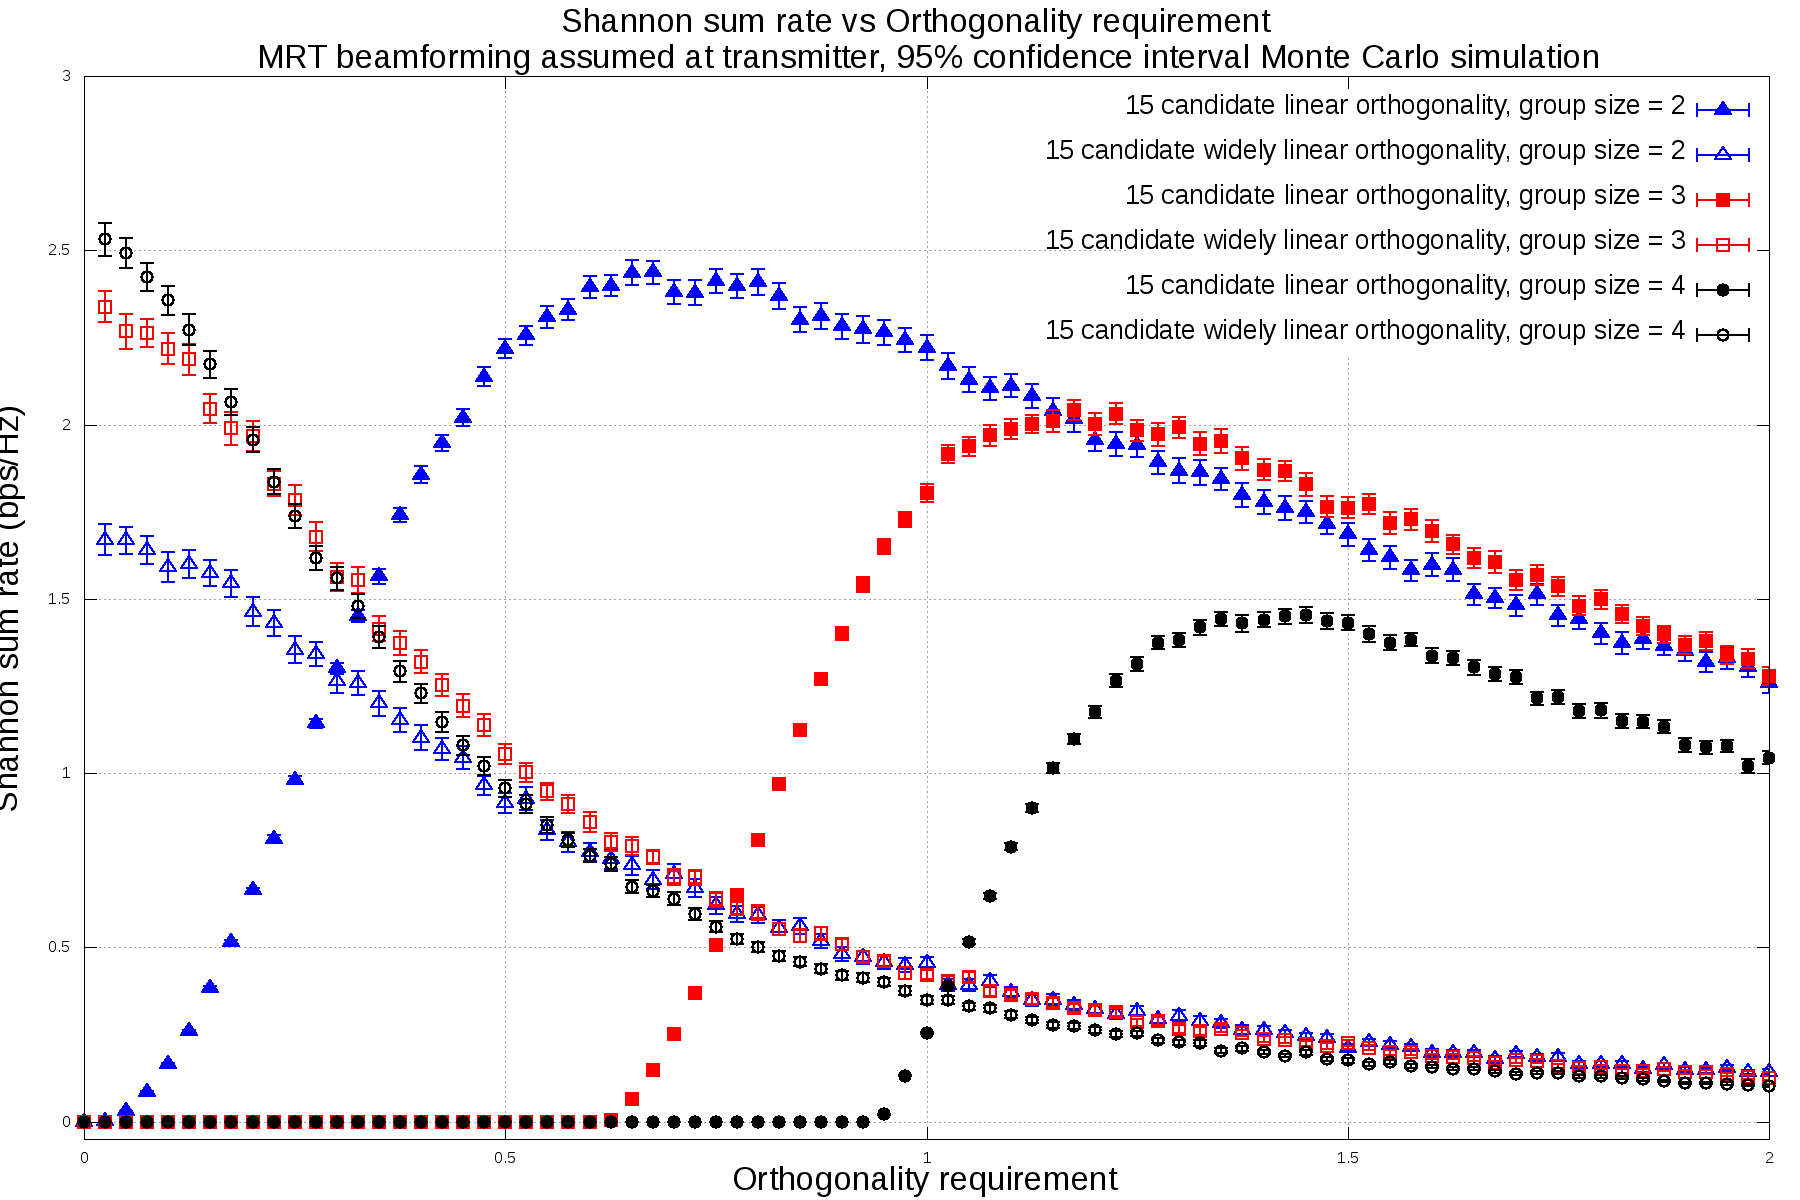
\includegraphics[width=24cm]{figs/15_candidate_mrt.png}\\
    \caption{Sum rate for single-dimensional and two-dimensional constellations, SUS group sizes set to 2, 3, 4. Number of candidate STAs for addition to SUS groups is held to 15.}
    \label{fig:15_candidate}
\end{sidewaysfigure}

Figure \ref{fig:30_candidate} shows  curves for two-dimensional constellation sum rates with $L = 30$ instead of 15. We see that the $K=3,4$ series now have higher maximum sum rate values. This result is expected: as the number of candidate STAs is increased, the probability of larger SUS groups existing for small values of $\epsilon$ increases. Increasing $L$ has less of an impact for $K=2$ because the existence probability has already saturated for small values of $\epsilon$.
\begin{sidewaysfigure}
    \centering
    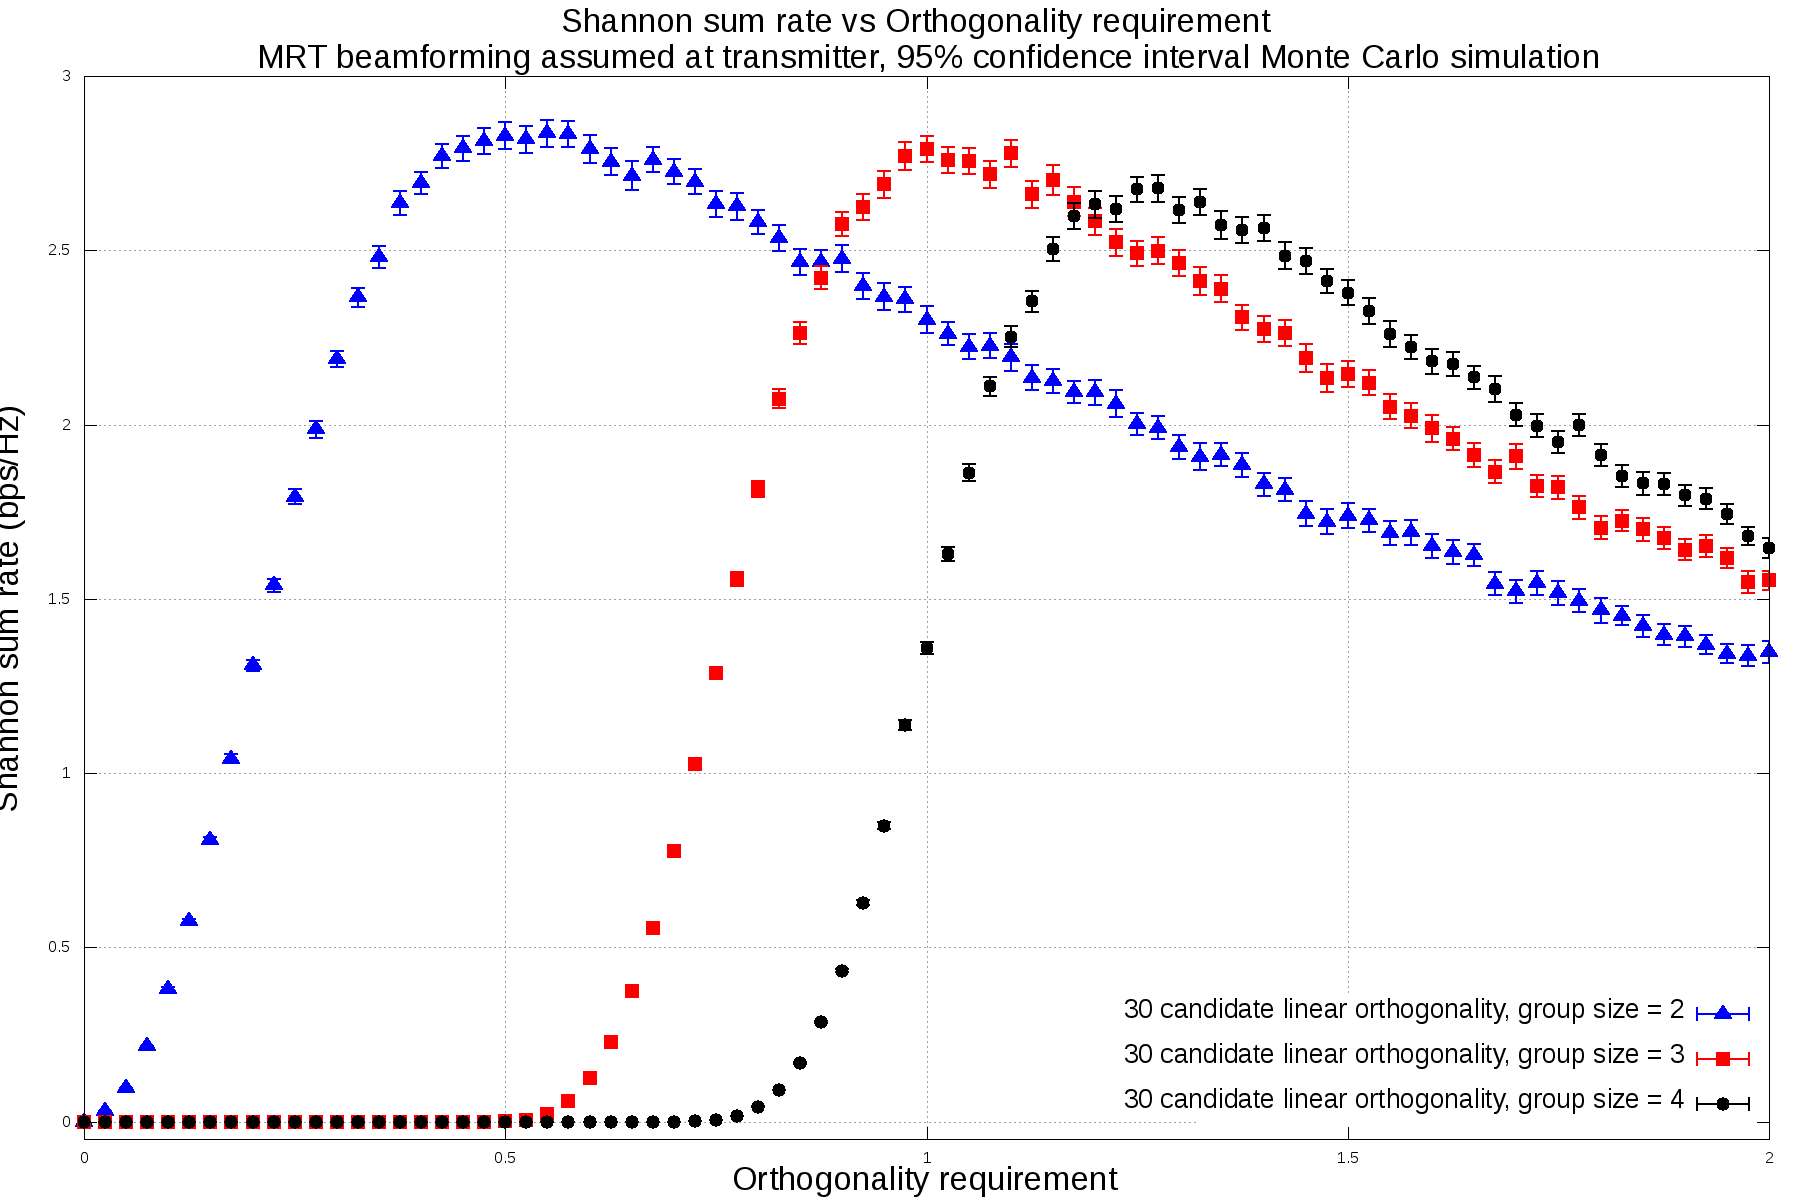
\includegraphics[width=24cm]{figs/30_candidate_mrt.png}\\
    \caption{Sum rate for two-dimensional constellations, SUS group sizes set to 2, 3, 4. Number of candidate STAs for addition to SUS groups is held to 30.}
    \label{fig:30_candidate}
\end{sidewaysfigure}

	%\section{Appendices}
	    %\subsection{Notes on Gamma-distributed variables}
	    %    \input{app/gamma_dist.tex}
    \newpage	
 	\begingroup
 		\renewcommand{\section}[2]{}%
 		\bibliographystyle{IEEEtran}
 		\bibliography{references}
 	\endgroup
\end{document}

Imported from Another project/review.tex, at 3:21 pm Today

 
